\documentclass[hidelinks,a4paper, 12pt]{article}
\usepackage[french]{babel}
\usepackage[utf8]{inputenc}
\usepackage[T1]{fontenc}
\usepackage{lmodern}
\usepackage{graphicx}
\usepackage{hyperref}
\usepackage{listings}
\usepackage{color}
\usepackage{svg}
\usepackage{cleveref}
\usepackage{subfig}
\usepackage{gensymb}
\usepackage{slashbox}
\usepackage{pgfplots}
\usepackage{pgfplotstable}
\usepackage{siunitx}
\usepackage{xcolor,colortbl}
\makeatletter
\pgfplotsset{
	/tikz/min node/.style={
		anchor=north
	},
	mark min/.style={
		point meta rel=per plot,
		visualization depends on={x \as \xvalue},
		scatter/@pre marker code/.code={
			\ifx\pgfplotspointmeta\pgfplots@metamin
			\def\markopts{}
			\else
			\def\markopts{mark=none}
			\fi
			\expandafter\scope\expandafter[\markopts,every node near coord/.style=green]
		},
		scatter/@post marker code/.code={
			\endscope
		},
		scatter,
	},
}
\usepackage[titletoc,title]{appendix}
\lstset{language=C,rangeprefix=//---------------,rangesuffix=----------------,includerangemarker=false,columns=spaceflexible,extendedchars=true,showspaces=false,showstringspaces=false,inputencoding=ansinew,tabsize=4,frame=shadowbox,morecomment=[is]{\#ifdef}{\#endif},morecomment=[is]{/*}{*/}}
\title{ La skip-list }
\author{Steve Zaretti}

\begin{document}
	
	\maketitle
	\newpage
	\tableofcontents
	\newpage
	
	\section{Introduction}
	En informatique, il est courant de vouloir enregistrer des données quelconques. Une structure de données est une représentation logique de ces données. La manière de représenter les données permet de résoudre différents problèmes. Une structure précise peut être plus performante pour un cas précis ou, au contraire, être très peu performante. D’autre part, une meilleure organisation de l'information peut aussi réduire de façon significative la complexité d’un algorithme.
	
	Il existe un grand nombre de structures de données, toutes proposent aux concepteurs de logiciel deux fonctionnalités standards : enregistrer et récupérer un renseignement. Selon l’approche employée pour la représentation logique, les performances seront différentes. Certaines structures de données offrent la possibilité de récupérer le premier élément en temps constant, au détriment du temps d’accès aux autres éléments. Alors que d’autres permettent un accès en temps constant à chacun des éléments en dépit d’une durée plus longue pour l’enregistrement d'une information.
	
	\subsection{Liste chaînée}\label{linkList}
	Une liste chaînée (\cref{LinkedList}) est une structure de données de taille variable. Le principe est que chacun des éléments de cette liste contient une référence vers l'élément suivant. Cette pratique facilite l'insertion et la suppression des éléments, au détriment de la rapidité de la recherche.
	
	Une liste chaînée peut aussi être triée, ce qui porte des conséquences sur ses performances. Une insertion devient plus compliquée, car il faut rechercher, avant tout, où placer l'élément dans la liste afin de garder la structure cohérente.
	
	La recherche dans une liste chaînée s'effectue élément par élément: si ce n'est pas le premier élément de la liste, il faut regarder le second. Si ce n'est pas celui-ci, il faut alors regarder celui d'après jusqu'à ce que l'élément recherché soit trouvé ou qu'il n'y ait pas d'élément suivant. Dans le cas d'une liste chaînée croissante, la recherche peut s'arrêter plus tôt: si l'élément que l'on regarde est plus grand que celui qui est recherché.
	
	\begin{figure}[h]
		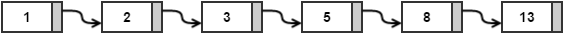
\includegraphics[width=\textwidth]{img/linkedList}
		\caption{Liste chaînée ordonnée}
		\label{LinkedList}
	\end{figure}
	
	Par exemple dans la \cref{LinkedList}, pour rechercher l'élément contenant la valeur 6. La recherche commence par la gauche de la liste. 1 est plus petit que 6, il faut alors regarder l'élément suivant. 2, 3, et 5 sont toujours plus petits que 6, la recherche progresse élément par élément. Par contre, 8 est plus grand que 6. La recherche se termine, infructueuse.
	
	\subsubsection*{Les alternatives}
	Il existe de nombreuses alternatives aux listes chaînées pour trouver un élément plus rapidement: les tables de hachage (\cref{hashing}), les arbres binaires de recherche (\cref{tree}), etc. Mais certaines séquences d'insertions peuvent être catastrophiques. Par exemple, insérer des éléments croissants dans un arbre binaire de recherche provoque un rééquilibrage de l'arbre. En revanche, si les éléments sont insérés de façon aléatoire, l'équilibrage devient plus rare. Plus d'informations dans la \cref{compare}.

	Grâce aux probabilités, les \og skip-list \fg{} (\cref{skip}) bénéficient d'un atout majeur: il ne faut pas les rééquilibrer. Mieux encore, la skip-list utilise des algorithmes plus simples que ses concurrents.
	
	\begin{figure}[h]
		\centering
		\subfloat[Table de hachage] {
			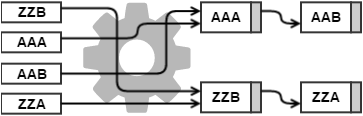
\includegraphics[scale=0.75]{img/hashing}
			\label{hashing}
		}
		\subfloat[Arbre binaire de recherche] {
			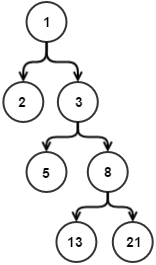
\includegraphics[scale=0.75]{img/tree}
			\label{tree}
		}
		\caption{Différentes structures de données}
	\end{figure}
	\begin{figure}
		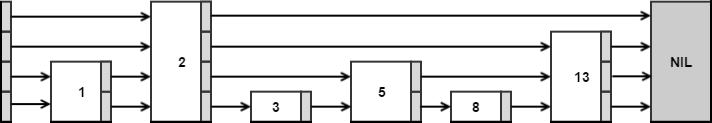
\includegraphics[width=\textwidth]{img/skip}
		\caption{Skip-list}
		\label{skip}
	\end{figure}
	
	\newpage
	\subsection{Skip-List}
	Tout comme un dictionnaire, une skip-list permet de récupérer la définition d'un terme recherché \textit{(dit clé)}. Cette recherche est rapide, car les éléments \textit{(dit nœud)} présents dans un dictionnaire sont triés et il est possible de commencer une exploration à un endroit précis.
	Une skip-list bénéficie des avantages de la liste chaînée (\cref{linkList}), en limitant fortement ses inconvénients. Cette structure de données utilise les chaines de façon parallèle. Une fonction basée sur des probabilités permet de déterminer la hauteur de la chaine. Plus cette hauteur est élevée, moins la liste contient d'éléments. Une couche haute est donc un accès plus rapide vers des éléments plus loin dans la liste.
	
	\begin{figure}[h]
		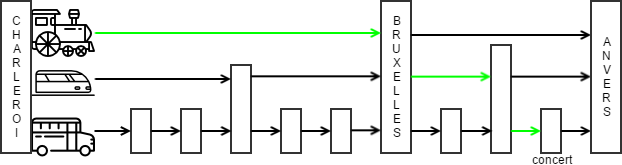
\includegraphics[width=\textwidth]{img/metaphore}
		\caption{Métaphore d'une skip-list par un réseau de transport en commun}
		\label{skip-meta}
	\end{figure}
	
	Afin d'illustrer la skip-list, il faut l'imaginer comme un réseau de transport en commun idéal où le temps d'attente des correspondances est nul. Un nœud dans la skip-list est un arrêt obligatoire dans lequel un passager peut changer de moyen de locomotion. La couche la plus basse dans la skip-list peut-être interprétée comme un bus. Il s'arrête à chacun de ses arrêts prévus, son temps de parcours est très lent. La couche n\degree2, plus rapide, est un métro. La couche n\degree3, un train. Si un passager souhaite aller voir un concert à Bruxelles alors qu'il est à la gare de Charleroi, il ne va pas faire le trajet en bus. Il est tout naturel et plus rapide dans ce cas de prendre dans un premier temps le train, puis le métro afin qu'il se rapproche le plus près possible du concert. Si le dernier arrêt de métro n'a pas permis d'accéder à la salle du concert, seulement dans ce cas le passager doit emprunter le bus.
	
	\subsubsection*{Définition}
	La hauteur maximale d'une skip-list est définie lors de sa création. Si $p=\frac{1}{2}$, il est conseillé d'utiliser $log_2(n)$ où $n$ est le nombre d'éléments théoriques présents dans la liste (voir \cref{perf}).
	
	L'insertion dans la liste utilise une fonction basée sur la probabilité $p$ afin de définir sa hauteur maximale. Si $p$ vaut $\frac{1}{2}$, ça signifie que le nœud a une probabilité de $\frac{1}{2}$ d'être de niveau 1, et a une probabilité $\frac{1}{2}$ d'être plus haut que 1. Un nœud de hauteur $h$ possède $h$ pointeur. Un nœud de hauteur 3 a donc un accès au nœud suivant de hauteur 3, ainsi que celui de hauteur 2 et 1.
	
	En raison des probabilités, les nœuds supérieurs possèdent un pointeur vers un nœud plus avancé dans la liste. Une couche supérieure est donc une voie plus rapide. Ainsi, la couche la plus haute contient les plus grands sauts, et la couche la plus basse permet d'accéder à chacun des éléments.
		
	Le parcours d'une skip-list se fait de haut en bas, et de gauche à droite. Si la clé de l'élément suivant sur une couche est plus grande que celle qu'on recherche, celle-ci continue sur une voie inférieure. (Voir \cref{SkipSearch1} et \cref{SkipSearch2} )	
	
	\begin{figure}[h]
		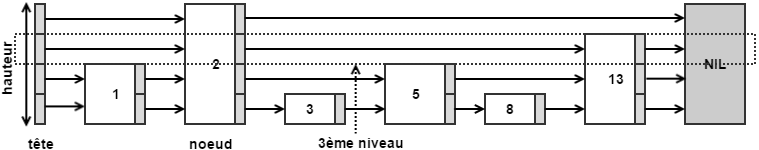
\includegraphics[width=\textwidth]{img/struct}
		\caption{Structure d'une skip-list}
		\label{StructSkip}
	\end{figure}
	
	\subsection{La hauteur}
	La notion de hauteur est très importante dans une skip-list. En effet, celle-ci permet de définir à combien de nœuds un élément est attaché. Si trop d'éléments possèdent la même hauteur, la recherche devient trop lente.	Cette hauteur est définie à l'aide d'une fonction aléatoire. Celle-ci ne dépend ni de la clé de l'élément ni de sa valeur. Dans le cas où $p=\frac{1}{2}$, la fonction aléatoire doit être définie pour qu'un élément de hauteur $h$ possède le double de probabilités qu'un élément de hauteur $h+1$. Ainsi, si un nœud de hauteur 1 a une probabilité $p$ de $0.5$ alors le niveau 2 a une probabilité de $0.25$.
		
	\newpage
	\section{Les algorithmes}
	Une skip-list a besoin d'avoir un pointeur vers sa tête. La liste doit connaitre le nombre de niveaux actuellement utilisés $(level)$. Selon les implémentations, il est possible de définir la hauteur maximale $(levelMAX)$. Il est aussi possible de changer le paramètre $(p)$ de probabilité de création d'une nouvelle couche. La variation de ces deux derniers paramètres est étudiée dans le chapitre \nameref{perf}.
	Un nœud contient une clé $key$ , une valeur $value$ ainsi qu'un tableau de pointeur vers les nœuds suivants $forward$. Il n'est pas nécessaire d'enregistrer la hauteur d'un nœud dans celui-ci.
	\lstinputlisting[linerange=BEGINSKStruct-ENDSKStruct]{SkipList/SkipList.h}
	
	L'initiation se fait de la manière suivante:
	\begin{itemize}
		\item La hauteur maximale est déterminée par le nombre d'éléments totaux $(n)$ présents dans la liste. Pour des questions de rapidité, la valeur $log_\frac{1}{p}(n)$ est recommandée.
		\item Création d'un élément $NIL$ possédant une clé plus grande que le maximum autorisé. Cet élément est aussi appelé \textit{élément bidon}.
		\item Définition de ses pointeurs $forward$ vers lui-même.
		\item Le nombre de voies actuelles est fixé à 1.
		\item Le pointeur de tête est défini par cet élément $NIL$.
	\end{itemize}
	\emph{La création d'une skip-list en langage C figure en annexe.}
	
	\begin{figure}[h]
		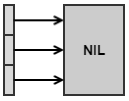
\includegraphics[scale=0.95]{img/init}
		\caption{Initialisation d'une skip-list}
		\label{SkipInit}
	\end{figure}
	
	\newpage
	\subsection{La recherche}
	De manière générale, pour rechercher dans une skip-list il suffit de commencer par le niveau le plus haut et d'effectuer une recherche élément par élément. Si l'élément suivant devient plus grand que celui recherché, il suffit alors de descendre d'un niveau dans la liste.
	
	Algorithmiquement parlant, la recherche d'un élément s'exécute de la façon suivante:
	\begin{enumerate}
		\item Commencer l'exploration de la liste par l'élément en tête, et se positionner sur la plus haute voie.
		\item Sur la voie actuelle, notre clé est-elle plus grande que celle de l'élément suivant?
		\item Si oui, se positionner sur cet élément et retourner en 2.
		\item Si non, existe-t-il une voie inférieure?
		\subitem Si oui, descendre d'une voie et retourner en 2. 
		\subitem S'il n'existe pas de voie inférieure, continuer en 5.
		\subitem
		\item Si la clé de l'élément suivant correspond à celle qui est recherchée: l'élément a été trouvé.
		\item Sinon, l'élément n'a pas été trouvé.
	\end{enumerate}
	
	\emph{L'algorithme écrit en langage C figure en annexe.}
	
	\paragraph*{Comment rechercher l'élément 8 dans l'exemple de la \cref{SkipSearch1}?}
	\begin{itemize}
		\item Se positionner sur la couche la plus haute: La 4ème voie.
		\item 8 est-il plus grand que 2 ? Oui, se positionner sur le nœud 2.
		\item 8 est-il plus grand que $+\infty$ \textit{(NIL)}? Non, descendre sur la 3ème voie.
		\item 8 est-il plus grand que 13  ? Non, descendre sur la 2ème voie.
		\item 8 est-il plus grand que 5 ? Oui, se positionner sur le nœud 5.
		\item 8 est-il plus grand que 13 ? Non, descendre sur la 1ère voie.
		\item 8 est-il plus grand que 8 ? Non, il n'existe pas de voie plus basse.
		\item 5 est le dernier nœud parcouru. L'élément suivant sur la voie 1 est 8. 8 est-il l'élément recherché? Oui, la recherche est concluante.
	\end{itemize}
	\begin{figure}[h]
		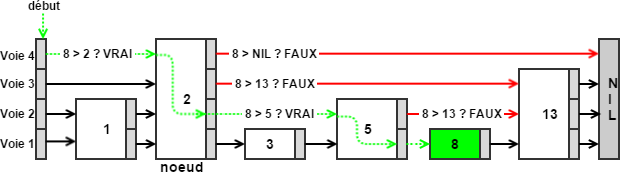
\includegraphics[width=\textwidth]{img/search}
		\caption{Recherche de l'élément 8 dans une skip-list}
		\label{SkipSearch1}
	\end{figure}
	
	\newpage
	\paragraph*{Comment rechercher l'élément 8 dans \cref{SkipSearch2}?}
	
	\begin{itemize}
		\item Se positionner sur la couche la plus haute: La 4ème voie.
		\item 8 est-il plus grand que 2 ? Oui, se positionner sur le nœud 2.
		\item 8 est-il plus grand que $+\infty$ \textit{(NIL)}? Non, descendre sur la 3ème voie.
		\item 8 est-il plus grand que 13  ? Non, descendre sur la 2ème voie.
		\item 8 est-il plus grand que 5 ? Oui, se positionner sur le nœud 5.
		\item 8 est-il plus grand que 13 ? Non, descendre sur la 1ère voie.
		\item 8 est-il plus grand que 8 ? Non, il n'existe pas de voie plus basse.
		\item 5 est le dernier nœud parcouru. L'élément suivant sur la voie 1 est 9. 9 est-il l'élément recherché? Non, la recherche est infructueuse.
	\end{itemize}
	\begin{figure}[h]
		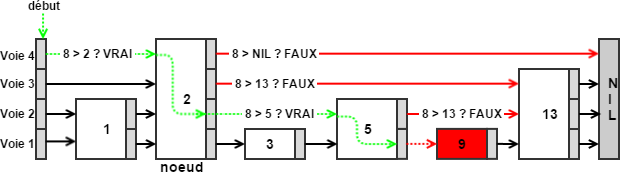
\includegraphics[width=\textwidth]{img/search2}
		\caption{Recherche de l'élément 8 dans une skip-list}
		\label{SkipSearch2}
	\end{figure}
	
	
	\newpage
	\subsection{L'insertion}
	L'insertion d'une entrée dans une skip-list est essentiellement la même chose que la recherche. À l'exception qu'un tableau $update$, de taille identique à la hauteur de la liste, est utilisé pour mémoriser les pointeurs de chaque élément avant de descendre d'un niveau. Ce tableau est utilisé pour mettre à jour les liens nécessaires pour que la structure de données reste cohérente.
	
	Algorithmiquement parlant, l'insertion d'un élément dans une skip-list s'effectue de la façon suivante:
	
	\begin{enumerate}
		\item Commencer l'exploration de la liste par l'élément en tête, et se positionner sur la plus haute voie.
		\item Sur la voie actuelle, notre clé est-elle plus grande que celle de l'élément suivant?
		\item Si oui, se positionner sur cet élément et retourner en 2.
		\item Si non, existe une voie inférieure? 
		\subitem Si oui, marquer ce pointeur, descendre d'une voie et retourner en 2.
		\subitem Si non, continuer en 5.
		\subitem 
		\item Si la clé de l'élément suivant correspond à celle qui est recherchée: modifier la valeur de l'élément par celle de la valeur à insérer. \textbf{FIN}.
		\item Sinon, appeler la fonction de probabilité pour récupérer le niveau $n$.
		
		\item Si $n$ est plus grand que la hauteur $h$ de la liste: mettre à jour les pointeurs supérieurs marqués à $h$ vers $NIL$. Ensuite, définir la hauteur maximum actuelle $h$ à $n$.
		\item Créer le nœud $x$ de hauteur $n$.
		
		\item Pour toutes les voies plus petites ou égales à $n$.
		\subitem  Mettre à jour les pointeurs de $x$ vers l'élément suivant de l'élément marqué. Modifier les pointeurs de l'élément marqué vers $x$.
		
		\item \textbf{FIN}.
	\end{enumerate}
	\emph{L'algorithme écrit en langage C est présenté en annexe.}
	
	\newpage
	\paragraph*{Comment insérer l'élément 5 dans \cref{SkipInsert2}?}
	\begin{itemize}
		\item Se positionner sur la couche la plus haute: La 4ème voie.
		\item 5 est-il plus grand que 2 ? Oui, se positionner sur le nœud 2.
		\item 5 est-il plus grand que $+\infty$ \textit{(NIL)}? Non, enregistrer ce lien en mémoire, puis descendre sur la 3ème voie.
		\item 5 est-il plus grand que 13 ? Non, enregistrer ce lien en mémoire, puis descendre sur la 2ème voie.
		\item 5 est-il plus grand que 13 ? Non, enregistrer ce lien en mémoire, puis descendre sur la 1ère voie.
		\item 5 est-il plus grand que 3 ? Oui, se positionner sur le nœud 3.
		\item 5 est-il plus grand que 8 ? Non, enregistrer ce lien en mémoire, il n'existe pas de voie plus basse.
		\item 5 est le dernier nœud parcouru. L'élément suivant sur la voie 1 est 8. Est-il l'élément recherché? Non, on crée un nouvel élément. Générer une hauteur aléatoire: hauteur 2.
		\item Ajouter un lien du nouvel élément 5 en voie 1. Ce lien doit pointer vers l'élément du lien enregistré à cette même voie. Il s'agit de l'élément 8.
		\item Modifier ce lien enregistré en voie 1 (de l'élément 3 vers l'élément 8) pour qu'il pointe vers ce nouvel élément 5.
		\item Ajouter un lien du nouvel élément 5 en voie 2. Ce lien doit pointer vers l'élément du lien enregistré à cette même voie. Il s'agit de l'élément 13.
		\item Modifier ce lien enregistré en voie 2 (de l'élément 2 vers l'élément 13) pour qu'il pointe vers ce nouvel élément 5.
		\item FIN.
	\end{itemize}
	\begin{figure}[h]
		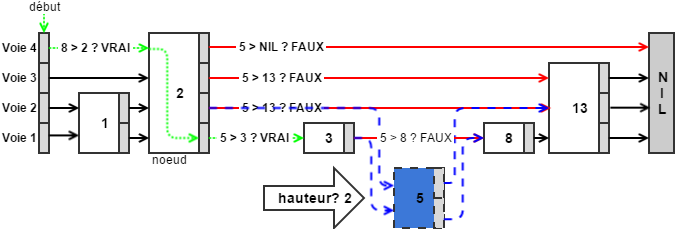
\includegraphics[width=\textwidth]{img/insert2}
		\caption{Insertion dans une skip-list}
		\label{SkipInsert2}
	\end{figure}
	
	\newpage
	\subsection{La suppression}
	La suppression d'un élément dans une skip-list s'effectue de la façon suivante:
	\begin{enumerate}
		\item Commencer l'exploration de la liste par l'élément en tête, et se positionner sur la plus haute voie.
		\item Sur la voie actuelle, notre clé est-elle plus grande que celle de l'élément suivant?
		\item Si oui, se positionner sur cet élément et retourner en 2.
		\item Si non, existe une voie inférieure? 
		\subitem Si oui, marquer ce pointeur, descendre d'une voie et retourner en 2.
		\subitem Si non, continuer en 5.
		\subitem 
		\item Si la clé de l'élément suivant ne correspond pas à celle qui est recherchée, \textbf{FIN}.
		\item Pour toutes les voies plus petites ou égales à $n$.
		\subitem  Mettre à jour les pointeurs marqués vers l'élément suivant de l'élément trouvé.	
		\item Supprimer l'élément trouvé.
		\item Si l'élément de tête de la hauteur actuelle de la liste pointe vers $NIL$, diminuer la hauteur actuelle de la liste de 1. Répéter l'opération si possible.
		\item \textbf{FIN}.
	\end{enumerate}
	\emph{L'algorithme écrit en langage C figure en annexe.}
	
	\newpage
	\paragraph*{Comment supprimer l'élément 5 dans la \cref{SkipDelete}?}
	\begin{itemize}
		\item Se positionner sur la couche la plus haute: La 4ème voie.
		\item 5 est-il plus grand que 5? Non, enregistrer ce lien en mémoire, puis descendre sur la 3ème voie.
		\item 5 est-il plus grand que 2 ? Oui, se positionner sur le nœud 2.
		\item 5 est-il plus grand que 5? Non, enregistrer ce lien en mémoire, puis descendre sur la 2ème voie.
		\item 5 est-il plus grand que 5? Non, enregistrer ce lien en mémoire, puis descendre sur la 1ière voie.
		\item 5 est-il plus grand que 3 ? Oui, se positionner sur le nœud 3.
		\item 5 est-il plus grand que 5 ? Non, enregistrer ce lien en mémoire, il n'existe pas de voie plus basse.
		\item35 est le dernier nœud parcouru. L'élément suivant sur la voie 1 est 5. Est-il l'élément recherché? Oui, mettre à jour les pointeurs enregistrés sur les voies 4 et 3 vers NIL. Mettre à jour les pointeurs enregistrés sur les voies 2 et 1 vers le nœud 13.
		\item Supprimer l'élément 5.
		\item Diminuer la hauteur actuelle de la liste à 3 car la voie 4 pointes vers $NIL$.
		\item FIN.
	\end{itemize}
	\begin{figure}[h]
		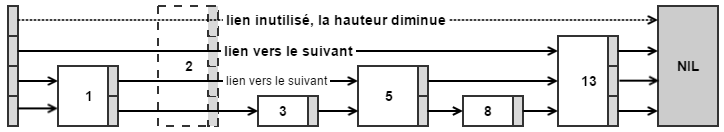
\includegraphics[width=\textwidth]{img/delete}
		\caption{Suppression de l'élément 5 dans une skip-list}
		\label{SkipDelete}
	\end{figure}
	
	\newpage
	\section{Analyse des performances}\label{perf}
	La caractéristique majeure de la skip-list est l'aléatoire. L'insertion d'un élément nouveau utilise une hauteur qui est déterminée par le hasard. De ce fait, une même séquence produira une liste différente.
	
	De par sa nature probabiliste, on suppose que l'utilisateur n'aura pas un comportement à vouloir dégénérer volontairement la liste. C'est-à-dire que les performances peuvent être dégradées en retirant consciemment les éléments après avoir inspecté leur hauteur. Si l'utilisateur supprime tous les nœuds de hauteur $h>1$, le pire scénario de la skip-list équivaut à une liste chaînée classique.
	
	Le temps requis pour exécuter l'insertion et la suppression dans une skip-list est prédominé par le temps de la recherche d'un élément. Ces deux derniers n'ont qu'un coût supplémentaire constant par rapport à la hauteur de la liste; alors que le coût de la recherche est proportionnel à la longueur du chemin à parcourir.
	
	
	\subsection{Analyse pour $p=\frac{1}{2}$}
	Pour une variable aléatoire $p=\frac{1}{2}$ et une skip-list de taille infinie, celle-ci tend à ce que chacun des niveaux possèdent $\frac{1}{2}$ moins d'éléments. Ainsi, le niveau 1 contient $n$ élément, le niveau 2 $\frac{n}{2}$, le niveau 3 $\frac{n}{4}$, ..., un élément à hauteur $h$: $\frac{n}{{2}^{h-1}}$.
	
	Par conséquent, le nombre total de liens dans une skip-list équivaut à: \[n+\frac{n}{2}+\frac{n}{4}+\frac{n}{8}+\dots = \sum_{h=1}^{+\infty}\frac{n}{{2}^{h-1}}=2n\] Ce qui signifie qu'en moyenne un élément dans une skip-list possède 2 liens. On peut donc déduire qu'en moyenne le nombre de fois que l'on avance dans la liste à un niveau précis équivaut au nombre de liens divisé par le nombre d'éléments, soit $\frac{2n}{n}=2$. En effet, chaque nœud examiné à un niveau $i$, ne peut pas appartenir à un niveau $i+1$. Pour chaque clé apparaissant au niveau $i$, la probabilité qu'elles n'apparaissent pas au niveau $i+1$ est $\frac{1}{2}$. En d'autres mots, si le niveau $i$ contient $k$ éléments, le niveau $i+1$ en contiendra $k*p$ éléments.
	
	\newpage
	La probabilité qu'un élément soit de hauteur $i$ est de ${p^{i-1}*(1-p)} = \frac{1}{2^{i}} $. Le facteur $p$ est constant ($\frac{1}{2}$), la probabilité de la hauteur des clés est équiprobable. Si l'on additionne la probabilité de hauteur chacune des clés de la skip-list, et que l'on prend $h$ comme hauteur de la liste, on déduit la formule suivante.
	\[
		\frac{1}{{2}^{1}}+\frac{1}{{2}^{2}}+\frac{1}{{2}^{3}}+\dots+\frac{1}{{2}^{h}}
		= \sum _{i=1}^{h} ({\frac{1}{2}})^{i}
	\]
	\[
		\sum _{i=1}^{\infty} ({\frac{1}{2}})^{i} = \frac{1}{2} + \frac{1}{4} + \frac{1}{8} + \frac{1}{16} + ... = 1
	\]
	
	Il est possible d'estimer cette hauteur. Si $h$ tend vers l'infini, la série converge vers 1. Il est donc possible de rechercher une hauteur moyenne à laquelle il n'y a plus d'élément. Posons alors $h$ tel que ${(\frac{1}{2})}^h*n = 1$. 

	\[
		{(\frac{1}{2})}^{h}=\frac{1}{n}
		\iff h = \log_{\frac{1}{2}}(\frac{1}{n})
		\iff h = \log_{2}(n)
	\]
	
	L'algorithme de recherche possède 2 boucles imbriquées. La boucle la plus profonde permet d'avancer de gauche à droite dans la liste. Pour $p=\frac{1}{2}$, en moyenne celle-ci avance de $2$. La boucle supérieure quant à elle varie selon la hauteur de la liste. La hauteur est estimée, avec une forte probabilité, à $\log_{2} n $. Si l'on combine les 2 estimations, nous avons donc une forte probabilité que la recherche s'effectue en $\log_{2}( 2n )$ opérations, soit $\mathcal{O}(log(n))$.
	
	\subsection{Forte probabilité}
	La recherche pour $p=\frac{1}{2}$ s'effectue avec une forte probabilité en $\mathcal{O}(log(n))$. Mais cette valeur de "forte probabilité", quelle est-elle? Il est possible de le théoriser en posant des valeurs. Posons donc $\mathcal{O}(3log(n))$ comme temps de recherche maximum acceptable et calculons sa probabilité $P$ pour $n$ éléments.
	\[
		P \le {\frac{n}{2}}^{i}
		\longrightarrow P \le {\frac{n}{2}}^{log_2(n)} = 1
		\longrightarrow P \le {\frac{n}{2}}^{3log_2(n)} = \frac{1}{n^2}
	\]
	Ce qui signifie que si $n=1000$, il y a une probabilité d'une chance sur un million que la hauteur de la liste soit plus grande que prévu. De façon plus générale pour n'importe quelle constante $c>1$, $h$ est plus grand que $c log_2(n)$ est d'au plus $\frac{1}{n^{c-1}}$. Alors que la probabilité que  $h$ soit plus petit que $c log_2(n)$ est de $1-\frac{1}{n^{c-1}}$. Par conséquent, la hauteur d'une skip-list est définie avec une forte probabilité en $\log_{2}(n)$.
	
	
	\subsection{La hauteur}
	 Afin de calculer la probabilité qu'un nœud atteint un niveau précis $i$, il faut prendre un autre exemple que $p=\frac{1}{2}$. Avec $\frac{1}{4}$, nous pouvons calculer son niveau de cette façon: ${p^{i-1}*(1-p)} = \frac{1}{{4}^{i-1}}*(1-\frac{1}{4}) $. Ainsi, la fonction "getRandomLevel" de la skip-list peut être illustrée de cette façon.
	 
	 \begin{figure}[h]
	 	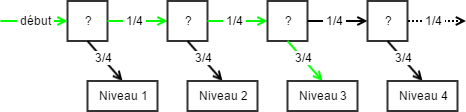
\includegraphics[width=\textwidth]{img/probatree}
	 	\caption{Arbre de probabilité}
	 	\label{ProbaTree}
	 \end{figure}
	 
	 \subsection{Généralisation}
	 Le raisonnement utilisé précédemment pour $p=\frac{1}{2}$ reste valable, quelle que soit la valeur de $p$, voir \cref{recap}. Le raisonnement qui effectue une sommation servant au calcul de lien dans une liste convergera vers $\frac{n}{p}$. Par contre, la somme des probabilités ($p^1 + p^2 + p^3 + ... + p^k$), converge toujours vers $\frac{p}{1-p}$ si $p<1$. 
	 
	 
	 \begin{table}[h]
	 \begin{tabular}{|l|c|c|}
	 	\hline
	 	Scénario & attendu & pire \\
	 	\hline
	 	Nombre d'éléments & $n$ & $n$ \\ 
	 	\hline
	 	Hauteur & $log_{\frac{1}{p}} n$ & $\infty$\footnotemark  \\ 
	 	\hline
	 	Nombre de liens & $n/p$ & $n*h$ \\ 
	 	\hline
	 	Recherche & $\mathcal{O}(\log n)$ & $\mathcal{O}(n)$ \\ 
	 	\hline
	 	Insertion & $\mathcal{O}(\log n)$ & $\mathcal{O}(n)$ \\
	 	\hline
	 	Suppression & $\mathcal{O}(\log n)$ & $\mathcal{O}(n)$\\
	 	\hline
	 \end{tabular}
	 \caption{Tableau récapitulatif}
	 \label{recap}
	 
	 \end{table}
	 
	\footnotetext{Les ordinateurs ne possèdent pas une mémoire infinie. C'est pourquoi à la création d'une skip-list, la hauteur maximale est bornée par la formule du cas attendu. Par conséquent, il est impossible d'avoir une hauteur infinie. }
	 	
	 
	
	\newpage
	\subsection{Expérimentation}
	
	Les expérimentations suivantes ont été réalisées sur un ordinateur Windows 10 64 bits possédant un AMD FX 8350 et 16Gb de RAM. Les tests ont été lancés $10^5$ fois, les résultats présentés sont la moyenne de tous les tests. Les très légères différences avec les résultats attendus peuvent s'expliquer par la façon dont un ordinateur génère des nombres aléatoires. On parle d'ailleurs de nombre "pseudo" aléatoire.
	
	L'algorithme utilisé pour générer les nombres aléatoires dans ces tests est \textit{xoroshiro128+}. Il a été développé par David Blackman et Sebastiano Vigna. Il s'agit de l'algorithme le plus rapide aujourd'hui. Il est intéressant d'utiliser un générateur rapide afin de déterminer la hauteur d'un élément de la skip-list. L'utilisation de la fonction \textit{rand} de \textit{stdlib} permet d'insérer $10^7$ éléments en $5.792$ secondes, alors que l'algorithme \textit{xoroshiro128+} permet d'en insérer autant en $4.014$ secondes. Cette différence de $30\%$ n'est pas négligeable.
	
	\begin{table}[h]
		\resizebox{\columnwidth}{!}{
			\begin{tabular}{|c|r|r|r|r|r|r|r|r|r|r|}
				\hline
				\backslashbox{p}{h} & 1 & 2 & 3 & 4 & 5 & 6 & 7 & 8 & 9 & 10 \\
				\hline
				4/5 & 1000.00 & 800.05 & 640.02 & 512.01 & 409.64 & 327.74 & 262.16 & 209.74 & 167.81 & 134.23 \\
				3/4 & 1000.00 & 749.97 & 562.52 & 421.83 & 316.34 & 237.25 & 177.98 & 133.45 & 100.10 & 75.07 \\
				2/3 & 1000.00 & 666.76 & 444.52 & 296.35 & 197.60 & 131.70 & 87.79 & 58.49 & 38.98 & 25.99  \\
				3/5 & 1000.00 & 600.00 & 360.00 & 216.02 & 129.61 & 77.77 & 46.66 & 28.00 & 16.79 & 10.06 \\
				1/2 & 1000.00 & 500.01 & 250.06 & 125.04 & 62.56 & 31.27 & 15.63 & 7.82 & 3.91 & 1.96 \\
				2/5 & 1000.00 & 399.96 & 160.02 & 64.01 & 25.60 & 10.23 & 4.09 & 1.63 & 0.00 & 0.00 \\
				1/3 & 1000.00 & 333.33 & 111.14 & 37.03 & 12.34 & 4.11 & 0.00 & 0.00 & 0.00 & 0.00 \\
				1/4 & 1000.00 & 249.97 & 62.48 & 15.63 & 3.90 & 0.00 & 0.00 & 0.00 & 0.00 & 0.00 \\
				1/5 & 1000.00 & 200.04 & 40.00 & 8.01 & 0.00 & 0.00 & 0.00 & 0.00 & 0.00 & 0.00 \\
				1/10 & 1000.00 & 100.01 & 10.02 & 0.00 & 0.00 & 0.00 & 0.00 & 0.00 & 0.00 & 0.00 \\
				1/20 & 1000.00 & 50.00 & 0.00 & 0.00 & 0.00 & 0.00 & 0.00 & 0.00 & 0.00 & 0.00 \\
				\hline
			\end{tabular}
		}
		\caption{Le nombre d'éléments par niveau en fonction de $p$}
		\label{tbRes1}
	\end{table}
	
	\subsubsection*{Variation de p}

	Afin de vérifier que le $p$ à bien l'effet voulu, il suffit de compter le nombre d'éléments existants à chaque niveau. S'il y a $n$ éléments à la hauteur 1, on s'attend à obtenir $np$ éléments de hauteur 2.
	
	Dans les faits, en essayant différentes valeurs pour une skip-list de 1000 éléments, on  peut obtenir les résultats présents dans la \cref{tbRes1}. Le résultat obtenu, correspond à notre espérance: $p$ influence correctement la hauteur de la liste et par conséquent son poids. 
	
	Une question plus intéressante à se poser serait: Quel est la meilleure valeur pour $p$ ? Choisir un petit nombre réduit le nombre de liens dans la liste. Cela a comme conséquence de pouvoir faire de plus grand saut, mais moins souvent. Par exemple avec $p=0.1$, il sera fort probable de faire des sauts d'une dizaine d'éléments. En revanche, choisir un grand nombre pour $p$, augmentera fortement le nombre de liens dans la skip-list. Celle-ci possède donc un grand nombre de hauteurs, et donc permet plus de sauts. Cela a comme conséquence de faire plus souvent des sauts, mais ils seront plus petits.
	 
	\begin{figure}[h]
		\centering
		\resizebox{0.8\columnwidth}{!}{
			\begin{tikzpicture}
			\begin{axis}[
				ymin=300,xmin=0.05,xmax=0.80,xtick distance=0.1,ytick distance=100,
				ylabel={Temps},
				xlabel=Valeur de $p$
			]
			\addplot+[smooth,mark min] table [x=p,y=1000] {data/pvar.dat};
			\addplot+[smooth,mark min] table [x=p,y=10000] {data/pvar.dat};
			\addplot+[smooth,mark min] table [x=p,y=100000] {data/pvar.dat};
			\addplot+[smooth,mark min] table [x=p,y=1000000] {data/pvar.dat};		
			\end{axis}
			\end{tikzpicture}
		}
		\caption{Vitesse d'exécution en fonction de $p$}
		\label{tbRes2}
	\end{figure}
	
	\section{Comparaisons avec d'autres structures}\label{compare}
	Dans la conception logicielle, choisir la bonne structure de données permet aux logiciels de s'exécuter plus rapidement. Laquelle présentera les meilleures performances? Quels sont les avantages et le prix à payer? Pour l'ensemble de ces tests, un logiciel de comparaisons doit être utilisé, spécialement développé pour ce projet.
	Il existe un grand nombre de méthodes différentes pour enregistrer des données au format "clé-valeur". Ces structures de données sont appelées des dictionnaires. Dans un dictionnaire de langue française, chacun des mots est associé à une définition. Ces mots sont triés par ordre alphabétique afin d'effectuer des recherches rapides. En informatique, c'est le même concept qui est utilisé: Chacune des clés (mots) correspond à une valeur (définitions). Les clés, quant à elles, seront structurées de façon organisée afin de pouvoir les trouver rapidement.
	
	\subsection{La table de hachage}
	La table de hachage est une structure de données qui fonctionne grâce à des listes chaînées. Le pointeur du premier élément est placé dans un vecteur. Ce vecteur est typiquement initialisé pour contenir 128 éléments. 
	
	Lors de l'insertion dans cette table, la clé est transformée à l'aide d'une méthode de "hachage". Cette dernière doit être capable de répartir efficacement les éléments tout en étant déterministe. C'est à dire, qu'insérer ou rechercher un élément ayant comme clé "4000" doit toujours atteindre la même case du vecteur. 
	
	Si 2 éléments doivent s'insérer dans la même case du vecteur, ceux-ci sont alors placés dans une liste chaînée. Par exemple si la clé "48" et la clé "24" ont comme résultat de la fonction de hachage 12; L'élément 24 sera le premier élément de la liste chaînée, suivi de 48.
	
	Lorsque trop d'éléments sont présents dans une même case, la table de hachage doit pouvoir agrandir la taille de son vecteur. Cette modification impose que chacun des éléments présents dans la table soient déplacés pour correspondre aux nouveaux indices calculés par la fonction de hachage. Le nombre maximum de collisions autorisées par case est typiquement 4, mais peut-être configuré autrement. Une table de hachage de 128 cases peut donc contenir 512 éléments. 
	
	\lstinputlisting[linerange=BEGINStruct-ENDStruct]{SkipList/HashTable.h}
	\lstinputlisting[linerange=BEGINStruct-ENDStruct]{SkipList/LinkList.h}
	
	\subsubsection*{Avantages}
	\begin{itemize}
		\item Rapidité d'insertion et de recherche
		\item Simple mise en place 
	\end{itemize}
	\subsubsection*{Inconvénients}
	\begin{itemize}
		\item La fonction de hachage doit être suffisamment efficace pour éviter les collisions.
		\item Réallocation et déplacement des éléments en cas de grand nombre de collisions.
		\item L'utilisation d'un vecteur pour la table, limite le nombre maximum d'éléments.
	\end{itemize}
	\subsubsection*{Performances}
	
	Afin de négliger la méthode de hachage pour ce test: les clés sont des entiers. La méthode de hachage reprend le reste de la division euclidienne de la clé par la taille de la table. Ainsi, il est possible d'utiliser l'intégralité de la table en minimisant les collisions. Il suffit alors d'insérer des clés de façon séquentielle (0, 1, 2, 3...).
	
	 \begin{table}[h]
	 	\begin{tabular}{|l|c|c|}
	 		\hline
	 		Scénario & attendu & pire \\
	 		\hline
	 		Recherche & $\mathcal{O}(1)$ & $\mathcal{O}(n)$ \\ 
	 		\hline
	 		Insertion & $\mathcal{O}(1)$ & $\mathcal{O}(2n)$ \\
	 		\hline
	 		Suppression & $\mathcal{O}(1)$ & $\mathcal{O}(n)$\\
	 		\hline
	 	\end{tabular}
	 	\caption{Tableau récapitulatif}
	 \end{table}
	
	\newpage
	\subsection{Les arbres binaires}\label{BinaryTree}
	Un arbre binaire de recherche est une structure de données dans laquelle chacun des éléments possède 2 sous éléments. On parle alors de "fils gauche" et de "fils droit". Ces derniers peuvent eux aussi à leur tour, posséder un fils gauche et droit. On parle dès lors, de structures récursives.
	
	\lstinputlisting[linerange=BEGINStruct-ENDStruct]{SkipList/Tree.h}
	
	Chacun des nœuds a donc 2 fils: le gauche contient un élément plus petit que son parent et le fils droit qui contient un élément plus grand que son parent. Par exemple, un nœud de valeur 5 aura comme fils gauche 3, et comme fils droit 13.
	
	Les recherches dans un arbre s'effectuent depuis la racine de l'arbre, soit le nœud le plus haut dans sa hiérarchie. Il faut ensuite comparer l'élément courant avec celui qui est recherché. S'il est plus grand, il faut descendre sur le fils droit, sinon sur le fils gauche. La recherche continue en comparant avec le dernier élément sélectionné. L'exploration de l'arbre s'arrête lorsque l'élément est trouvé, ou qu'un nœud n'a plus de fils.
	
	Les insertions et suppressions dans un arbre dépendent de la recherche. Il faut en effet garder la structure cohérente. Si un élément parent est supprimé, il faut être capable de le remplacer par un autre sans détériorer l'arbre.
	
	Les insertions séquentielles posent problème dans un arbre. En effet, dans une suite de nombres strictement croissants, chacun des nombres est par définition plus grand que son précédent. Par conséquent, de telles insertions dans un arbre provoqueront une dégradation significative des performances. Le nombre inséré étant plus grand que son précédent, celui-ci est toujours ajouté sur le fils droit. Le fils gauche n'est par conséquent jamais utilisé; ce qui transforme l'arbre en liste chaînée ordonnée.
	
	 \begin{table}[h]
	 	\begin{tabular}{|l|c|c|}
	 		\hline
	 		Scénario & attendu & pire \\
	 		\hline
	 		Recherche & $\mathcal{O}(\log n)$ & $\mathcal{O}(n)$ \\ 
	 		\hline
	 		Insertion & $\mathcal{O}(\log n)$ & $\mathcal{O}(n)$ \\
	 		\hline
	 		Suppression & $\mathcal{O}(\log n)$ & $\mathcal{O}(n)$\\
	 		\hline
	 	\end{tabular}
	 	\caption{Tableau récapitulatif}
	 \end{table}
	
	\subsubsection*{Avantages}
	\begin{itemize}
		\item Rapidité d'exécution, si l'arbre est équilibré
		\item Mise en place simple et rapide.
	\end{itemize}
	\subsubsection*{Inconvénient}
	\begin{itemize}
		\item L'insertion provoque rapidement un déséquilibre, ce qui détériore très fortement les performances
	\end{itemize}
	\subsubsection*{Performances}
	\begin{table}[h]
		\begin{tabular}{|l|c|c|}
			\hline
			Scénario & attendu & pire \\
			\hline
			Recherche & $\mathcal{O}(\log n)$ & $\mathcal{O}(n)$ \\ 
			\hline
			Insertion & $\mathcal{O}(\log n)$ & $\mathcal{O}(n)$ \\
			\hline
			Suppression & $\mathcal{O}(\log n)$ & $\mathcal{O}(n)$\\
			\hline
		\end{tabular}
		\caption{Tableau récapitulatif}
	\end{table}
	
	\subsection{Les arbres rouge-noir}
	Les arbres rouge-noir ou arbres bicolores, sont une amélioration des arbres binaires. Un nœud possède un attribut supplémentaire: sa couleur. Celle-ci peut être soit rouge, soit noir. Cela permet d'ajouter des contraintes dans l'arbre. Ces contraintes permettent de rééquilibrer l'arbre par des rotations. Il faut transformer l'arbre afin que le parent d'un nœud rouge soit noir. Mais aussi pour que le chemin de chaque feuille à la racine contienne le même nombre de nœuds noir.
	
	Lors de l'insertion, un nœud est rouge, mais en raison des transformations appliquées il peut devenir noir. Afin de garantir l'intégrité de la structure, il est possible qu'un nœud inséré ne soit pas une feuille, mais un parent. La recherche s'effectue exactement de la même façon qu'un arbre binaire.
	
	\lstinputlisting[linerange=BEGINStruct-ENDStruct]{SkipList/RBTree.h}
	
	\subsubsection*{Avantages}
	\begin{itemize}
		\item Rapidité d'exécution
		\item L'arbre est toujours équilibré
	\end{itemize}
	\subsubsection*{Inconvénients}
	\begin{itemize}
		\item Algorithme complexe à mettre en place en raison de nombreuses études de cas.
		\item Certaines séquences de nombres provoqueront un rééquilibrage systématique.
	\end{itemize}
	\subsubsection*{Performances}
	\begin{table}[h]
		\begin{tabular}{|l|c|c|}
			\hline
			Scénario & attendu & pire \\
			\hline
			Recherche & $\mathcal{O}(\log n)$ & $\mathcal{O}(\log n)$ \\ 
			\hline
			Insertion & $\mathcal{O}(\log n)$ & $\mathcal{O}(\log n)$ \\
			\hline
			Suppression & $\mathcal{O}(\log n)$ & $\mathcal{O}(\log n)$\\
			\hline
		\end{tabular}
		\caption{Tableau récapitulatif}
	\end{table}
	
	\subsection{La liste chaînée triée}
	Une liste chaînée (\cref{linkList}) est une simple chaine d'éléments. Chacun des éléments de cette liste contient une référence vers l'élément suivant. Lors d'une insertion, il faut rechercher où placer l'élément dans la liste afin de garder la structure triée.
	\lstinputlisting[linerange=BEGINStruct-ENDStruct]{SkipList/LinkList.h}
	
	\subsubsection*{Avantage}
	\begin{itemize}
		\item Algorithme extrêmement simple
	\end{itemize}
	\subsubsection*{Inconvénient}
	\begin{itemize}
		\item Très peu performant
	\end{itemize}
	\subsubsection*{Performances}
	\begin{table}[h]
		\begin{tabular}{|l|c|c|c|}
			\hline
			Scénario & Insertion en tête & Insertion en fin & Triée \\
			\hline
			Recherche & $\mathcal{O}(n)$ & $\mathcal{O}(n)$ & $\mathcal{O}(n)$ \\ 
			\hline
			Insertion & $\mathcal{O}(1)$ & $\mathcal{O}(n)$ & recherche +  $\mathcal{O}(1)$ \\
			\hline
			Suppression & $\mathcal{O}(n)$ & $\mathcal{O}(1)$ & recherche + $\mathcal{O}(1)$ \\
			\hline
		\end{tabular}
		\caption{Tableau récapitulatif}
	\end{table}
	

	\subsection{La Skip-List}
	\subsubsection*{Avantages}
	\begin{itemize}
		\item Rapidité d'exécution
		\item Algorithme simple
	\end{itemize}
	\subsubsection*{Inconvénient}
	\begin{itemize}
		\item Non déterministe
	\end{itemize}
	\subsubsection*{Performances}
	Les performances de la skip-list varient selon le paramètre $p$.
	\begin{figure}[h!]
		\centering
		\resizebox{\columnwidth}{!}{
			\begin{tikzpicture}
			\tikzstyle{every node}=[font=\tiny]
			
			\begin{axis} [
				axis y line*=left,
				ytick distance=0.1,
				width=7cm,height=3.5cm,
				legend style={font=\tiny,legend columns=-1},
				legend image post style={scale=0.3},
				ymin=0,ymax=0.5,xmin=0,xmax=128,
				ylabel=Temps en ms,
				ylabel near ticks,
				xlabel=Le nombre d'éléments,
				legend pos=north west
				]
			]
			\addplot+[mark=none, red, restrict x to domain=0:128] table [x=elem,y=sequence2] {data/skiplist.dat};
			\addplot+[mark=none, green, restrict x to domain=0:128] table [x=elem,y=sequence3] {data/skiplist.dat};
			\addplot+[mark=none, blue, restrict x to domain=0:128] table [x=elem,y=sequence4] {data/skiplist.dat};
			
			\addlegendentry{p=1/2}
			\addlegendentry{p=1/3}
			\addlegendentry{p=1/4}
			
			\end{axis}
			
			\end{tikzpicture}
		}
		\caption{Vitesse d'exécution d'une skip-list en fonction de $p$}
	\end{figure}
	\newpage
	\newpage
	
	\begin{figure}[h!]
		\centering
		\resizebox{\columnwidth}{!}{
			\begin{tikzpicture}
			\begin{axis} [
				axis y line*=left,
				ymin=0,ymax=10000,xmin=0,xmax=2000000,
				legend style={font=\tiny},
				ylabel=Temps en ms,
				ylabel near ticks,
				scaled x ticks={base 10:-3},
				scaled y ticks={base 10:-3},
				xlabel=Le nombre d'éléments,
				legend pos=south east,
			]
			\addplot+[mark=none, red] table [x=elem,y=sequence2] {data/skiplist.dat};
			\addplot+[mark=none, green] table [x=elem,y=sequence3] {data/skiplist.dat};
			\addplot+[mark=none, blue] table [x=elem,y=sequence4] {data/skiplist.dat};
			
			
			\addlegendentry{p=1/2}
			\addlegendentry{p=1/3}
			\addlegendentry{p=1/4}
			
			\end{axis}
			
			\end{tikzpicture}
		}
		\caption{Vitesse d'exécution d'une skip-list en fonction de $p$}
	\end{figure}
	
	\newpage
	\subsection{Comparaisons des performances d'insertions}
	Afin de comparer ces différentes structures de données, il est possible d'analyser leur temps d'exécution. Le tableau (\cref{compareAllTiming}) est la moyenne des résultats du logiciel de comparaison (option 3). Les temps affichés sont en $10^{-4}$ secondes. Ces temps ont été calculés à l'aide de l'instruction RDTSC présente sur les processeurs.
	
	
	
	\begin{table}[h]
		\resizebox{\columnwidth}{!}{
			\begin{tabular}{|S[table-format=8.0]|S[table-format=6.3]|S[table-format=6.3]|S[table-format=6.3]|S[table-format=6.3]|S[table-format=6.3]|}
				\hline
				{éléments} & {skip-list} & {link-list} & {tree} & {rb-tree} & {hashtable} \\
				\hline
				2 & 0.009 &  0.002 \cellcolor[gray]{0.8} & 0.003 & 0.003 & 0.005 \\
				4 & 0.016 &  0.004 \cellcolor[gray]{0.8} & 0.006 & 0.006 & 0.016 \\
				8 & 0.028 &  0.008 \cellcolor[gray]{0.8} & 0.010 & 0.010 & 0.023 \\
				16 & 0.055 &  0.017 \cellcolor[gray]{0.8} & 0.021 & 0.021 & 0.029 \\
				32 & 0.117 &  0.048 \cellcolor[gray]{0.8} & 0.050 & 0.054 & 0.068 \\
				64 & 0.228 & 0.096 & 0.093 \cellcolor[gray]{0.8} & 0.114 & 0.115 \\
				128 & 0.486 & 0.286 & 0.222 \cellcolor[gray]{0.8} & 0.243 & 0.234 \\
				256 & 0.995 & 0.898 & 0.436 \cellcolor[gray]{0.8} & 0.519 & 0.484 \\
				512 & 2.052 & 3.576 & 0.946 \cellcolor[gray]{0.8} & 1.083 & 0.973 \\
				1024 & 4.060 & 20.301 & 1.955 \cellcolor[gray]{0.8} & 2.228 & 2.567 \\
				2048 & 8.186 & 85.643 & 4.194 \cellcolor[gray]{0.8} & 4.573 & 5.930 \\
				4096 & 16.121 & 340.616 & 8.896 \cellcolor[gray]{0.8} & 9.749 & 12.966 \\
				8192 & 32.310 & 1375.928 & 20.218 \cellcolor[gray]{0.8} & 20.668 & 26.297 \\
				16384 & 65.748 & 5601.32 & 46.455 & 43.807 \cellcolor[gray]{0.8} & 52.140 \\
				32768 & 131.151 & 21765.4 & 111.791 & 93.318 \cellcolor[gray]{0.8} & 105.629 \\
				65536 & 273.893 & 957331 & 2124.687 & 202.261 \cellcolor[gray]{0.8} & 211.775 \\
				131072 & 570.276 &  & 26693 & 444.62 \cellcolor[gray]{0.8} & 464.442 \\
				262144 & 1189.503 &  & 191341 & 1013.92 \cellcolor[gray]{0.8} & 1086.389 \\
				524288 & 2372.10 &  &  & 2191.19 \cellcolor[gray]{0.8} & 2330.10 \\
				1048576 & 4843.64 &  &  & 4607.14 \cellcolor[gray]{0.8} & 5269.62 \\
				2097152 & 9998.07 &  &  & 9667.17 & 9458.14 {\cellcolor[gray]{0.8}} \\
				4194304 & 21672.3 &  &  & 19908.1 & 19841.2 {\cellcolor[gray]{0.8}} \\
				8388608 & 43113 &  &  & 42597 & 40985 {\cellcolor[gray]{0.8}} \\
				16777216 & 87929 &  &  & 88972 & 79736 {\cellcolor[gray]{0.8}} \\
				33554432 & 182116 &  &  & 213401 & 163435 {\cellcolor[gray]{0.8}} \\
				67108864 & 414702 &  &  & 544060 & 353891 {\cellcolor[gray]{0.8}} \\
				\hline
			\end{tabular}
		}
		\caption{Comparaisons du temps d'insertion}
		\label{compareAllTiming}
	\end{table}
	On peut en déduire qu'une liste chaînée est plus rapide que les autres structures, si le nombre d'éléments est inférieur à 64. Un arbre binaire de recherche est plus rapide, s'il y a moins de $2^{12}$ éléments. Ceci s'explique, car ces derniers ont une complexité $\mathcal{O}(log n)$ alors qu'une liste chaînée est en complexité $\mathcal{O}(n)$.
	
	Au-delà de $2^{12}$ éléments, l'arbre rouge-noir est plus rapide qu'un arbre binaire de recherche. Ce dernier commence à se déséquilibrer, ce qui ne garantit plus une performance optimale de $\mathcal{O}(log n)$. L'arbre rouge-noir quant à lui, possède des algorithmes permettant son rééquilibrage de façon automatique.
	
	À partir de $2^{22}$ éléments, la table de hachage devient plus rapide qu'un arbre rouge-noir. Il est aussi possible d'observer qu'au-delà de $2^{24}$ éléments, la skip-list devient plus rapide que l'arbre bicolore. Cela s'explique par le fait qu'une skip-list n'a pas besoin d'être rééquilibrée, quel que soit le nombre d'éléments insérés.
	
	\subsection{Différence entre les temps d'insertion}
	La rapidité d'insertion n'est pas la seule chose qui permet de privilégier une structure de données au lieu d'une autre. Par exemple, la skip-list ne doit pas être rééquilibrée alors qu'un arbre rouge-noir oui. À première vue, la skip-list a donc des temps d'insertions qui varient moins que les arbres bicolores. Les tables de hachage doivent s'agrandir au fur et à mesure des insertions. Le temps de la réallocation de la mémoire peut donc devenir un gros inconvénient, alors qu'elle était la plus rapide dans la plupart des cas. Le tableau (\cref{deltaTiming}) est la moyenne des résultats du logiciel de comparaison (option 4). Les temps affichés sont en $10^{-4}$ secondes, $2^{24}$ éléments ont été insérés.
	
	Les résultats du test révèlent que la table de hachage a eu le temps d'insertion le plus court. Ce qui est normal, étant donné que le temps d'accès à un vecteur par un système d'exploitation est très faible. Par contre, le temps d'exécution le plus long pour insérer un élément est presque 4 millions de fois plus grandes que le temps moyen. Le temps d'insertion est par conséquent extrêmement différent entre l'insertion de 2 données. Il n'est donc pas possible de se fier à cette structure de données pour des insertions prenant un temps uniforme.
	
	Comme vu dans la \cref{compareAllTiming}, le temps d'exécution de la skip-list est plus rapide que l'arbre bicolore pour insérer $2^{24}$ éléments. Les résultats du test affichent aussi que plus de la moitié des insertions étaient plus rapides pour la skip-list que l'arbre rouge-noir. Par contre en observant le 95ème centile du temps d'insertion, l'arbre rouge-noir était plus rapide.
	
	\begin{table}[h]
		\resizebox{\columnwidth}{!}{
			\begin{tabular}{|c|r|r|r|r|r|r|r|}
				\hline
				{structure} & {MIN} & {MAX} & {AVG} & {DEV} & {PC5} & {PC50} & {PC95} \\
				\hline
				skip-list & {\cellcolor{red!25}} 816 & {\cellcolor{green!25}} 1222713 & 1567 & {\cellcolor{green!25}} 5234 & {\cellcolor{green!25}} 1094 & {\cellcolor{green!25}} 1313 & {\cellcolor{red!25}}2004 \\
				hashtable & {\cellcolor{green!25}} 268 & {\cellcolor{red!25}}6079131241 & {\cellcolor{green!25}} 1534 & {\cellcolor{red!25}}1717849 & 308.0 & 639.3 & {\cellcolor{green!25}} 1218 \\
				RB-tree & 425 & 5763820 &  {\cellcolor{red!25}}1651 & 6055 &  {\cellcolor{red!25}}1182 &  {\cellcolor{red!25}}1467 & 1835 \\
				\hline
			\end{tabular}
		}
		\caption{Différence entre les temps d'insertion}
		\label{deltaTiming}
	\end{table}
	
	\section{Conclusion}
	La skip-list est une structure de données qui possède des algorithmes simples pouvant être implémentée en moins d'une heure. Ses performances sont très proches des arbres binaires de recherche, alors qu'elle n'a pas besoin d'être rééquilibrée. En raison des probabilités, il est possible qu'elle ne fonctionne pas de manière optimale. Cependant, plus le nombre d'éléments dans la liste est grand, plus la probabilité est faible et devient négligeable.
	
	La skip-list fonctionne comme une liste chaînée. Des pointeurs supplémentaires sont ajoutés selon la hauteur d'un nœud. Plus la hauteur du nœud est grande, plus celui-ci contient de liens vers l'un des éléments suivants dans la liste à cette même hauteur. La skip-list utilise un paramètre $p$ de probabilité pour influencer la hauteur. La valeur $p=\frac{1}{2}$ est conseillée, une valeur inférieure réduira sa place en mémoire.
	
	La probabilité $p=\frac{1}{2}$ est souvent associée avec l'analogie d'une pièce de monnaie. Pour savoir à quelle hauteur atteindra un nœud, il faut lancer une pièce. Chaque fois que le résultat correspond au côté face, il faut relancer la pièce. La hauteur d'un nœud correspond au nombre de lancé effectué.
	
	La recherche dans une liste commence sur le niveau le plus haut du premier élément de la liste. Cette recherche descend au niveau inférieur lorsque l'élément suivant est plus petit que la clé qui est recherchée.
	
	\vspace{1cm}
	En conclusion, la skip-list est une excellente alternative aux arbres binaires de recherche. Sa simplicité offre un champ d'action plus large que les algorithmes complexes des arbres équilibrés. La skip-list possède des fondements plus larges et plus efficaces que d'optimiser seulement le temps de recherche d'un élément.
	
	\nocite{1}
	\nocite{2}
	\nocite{3}
	\nocite{4}
	\nocite{5}
	\nocite{6}
	\nocite{7}
	\bibliographystyle{plain}
	\bibliography{rapport}
	
	\newpage
	\begin{appendices}
	\section{Représentation d'une Skip-List en langage C}
	Le code source est fourni sur le CD annexe. Il est aussi possible de le télécharger sur ce lien:
	\url{https://github.com/kossolax/UMONS/blob/master/SkipList/SkipList/SkipList.c}
	
	\section{Logiciel de comparaison}
	L'exécutable du logiciel est fourni sur le CD annexe. Il est aussi possible de le télécharger sur ce lien:
	\url{https://github.com/kossolax/UMONS/releases/download/v1/skipList.zip}
	
	\section{Répertoire GitHub}
	L'intégralité de ce document et du code source est disponible sur ce lien:
	\url{https://github.com/kossolax/UMONS/tree/master/SkipList}
	
	\end{appendices}
	
\end{document}